\section{Specifications}

\subsection{Cardiac signal}

The electrical potentials of the cardiac signal are acquired by various electrodes connected in the surface of the skin of the patient. Those combined generate the cardiac signal, as can be seen in the normal wave pattern of figure \ref{fig:cardiac_signal}, with voltage differences in the order of $1 \, mV$ between given points in the body \cite{khandpur2019compendium}.

\begin{figure}[h!] 
    \centering
    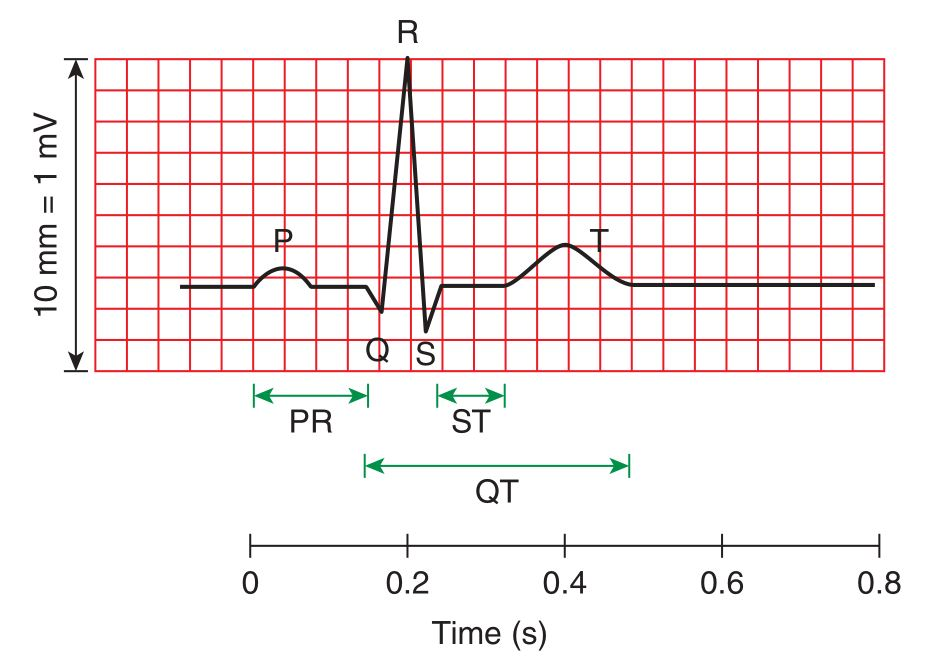
\includegraphics[width=9cm]{images/cardiac_signal.JPG}
    \caption{Normal waveform pattern of cardiac signal obtained in ECG. Source: \textcite{khandpur2019compendium}.}
    \label{fig:cardiac_signal} 
\end{figure}

Regarding the figure \ref{fig:cardiac_signal}, each letter has a proper meaning for each step in the cardiac cycle. Those are:

\begin{itemize}
    \item The P wave represents the depolarization of the atrial muscles;
    \item The QRS section is a combination of the atria repolarization between QR and the ventricles depolarization between RS;
    \item The T wave represents the repolarization of both ventricles;
\end{itemize}

The interval PR represents the actrial systole, of which the diastole lasts from R until the next P wave. The ventricular systole occurs between R until the end of the T wave and its diastole lasts until Q \cite{openstax}. 

The interval QRS representing the time taken by the heart impulse to travel from the inter ventricular system then through the walls of the ventricles is the most critical one when thinking in the design of an ECG machine since it has the higher frequency of all the cardiac signal and lasts about 0.05 to 0.1 seconds \cite{khandpur2019compendium}.

Those characteristics leads to a deeper specification of the ECG regarding the signal. \textcite{khandpur2019compendium} defines the frequency range of the signal varying from $0.05$ to $150 \, Hz$. By the Nyquist sampling theorem, it is recommended that the sampling frequency used in digitization to be at least two times the higher frequency in the signal, i.e $300 \, \text{samples}/s$. Despite this, \textcite{khandpur2019compendium} exerts that a sampling rate of $200 \, \text{samples}/s$ is satisfactory, yielding 12 to 20 samples for the QRS interval. Therefore the system designed in this work will attend to the Nyquist criteria and beyond, using a sampling frequency of $500 \, \text{samples}/s$. The disadvantage in this approach is that compared to the sampling frequency proposed by \textcite{khandpur2019compendium}, the present system will need $2.5 \times$ more space due its higher sampling frequency.

Regarding the bit resolution to store the cardiac signal, \textcite{khandpur1987handbook} suggests two approaches: to use low-noise and high-gain amplifiers, enabling the use of low-resolution 16-bit ADC; or using a low-gain amplifier with a high-resolution 24-bit ADC. The first approach will be used in this project for the sake of a more elaborated amplifier design and signal conditioning, instead just using a better ADC.

Since the arrangement of electrodes is not the main focus of this work, the system will stick with a bipolar leads arrangement. This arrangement uses two electrodes placed in the right and left arm to capture the signal and send to the input of an instrumentation amplifier and other electrode as reference placed in the left leg \cite{khandpur2019compendium}. This means that there is no need for a multiplexing system for multiples channels of electrodes, like in a typical 12-lead ECG \cite{zhang201212}.

\subsection{Associated noises}

In the chain of processing, the cardiac signal must be filtered in a way to remove certain noises and interference inherent to the data acquisition. The most common source are: interference from the power-lines (power grid) as a tone in $50/60 \, Hz$ (depending on the region of the globe); noise generated mechanically due to the contact between electrodes and skin, motion artefacts firing random derived from the patient movement and muscle contraction (voluntary or involuntary); additive white Gaussian noise (AWGN) derived from thermal sources; or electromagnetic interference from other electronics devices that can extends to the RF spectrum or higher \cite{khandpur1987handbook}.

It is essential to a ECG instrument to maintain clear of those noises and interference in a level of approximately $10 \, \mu V$ peak to peak to ensures ECG applications in diagnostics \cite{khandpur1987handbook}.

Each source of noise and interference can be treated in a specific manner.

\paragraph{Power-line interference} can be solved designing a Notch filter (reject band) with cutoff frequency set to $50/60 \, Hz$ (this project will validate the filter to $60 \, Hz$).

\paragraph{Baseline wanders and muscle contraction} are phenomena of low frequencies and they can be eliminated with the help of a high-pass filter. In the previous section the lower frequency defined to the cardiac signal was $0.05 \, Hz$, so a high-pass filter with this value as cutoff frequency should be able to remove those interference without risking rising too much the cutoff and attenuating the P or T waves \cite{khandpur2019compendium, khandpur1987handbook, murugappan2014development}. \textcite{sahin2020instrumentation} suggests the use of a $0.5 \, Hz$ cutoff frequency in a fourth order Butterworth filter, therefore allowing the use of a simpler filter with relaxed requirements and alerting that this cutoff may be tuned to meet the requirements. The $0.5 Hz$ cutoff frequency will be used in this project.

\paragraph{AWGN and electromagnetic interference} are phenomena of mainly high frequencies, therefore can be eliminated with a low-pass filter that might be designed with the anti aliasing filter. The anti aliasing filter is a analog and low order filter, but can also be used to eliminate electromagnetic interference since it has a frequency band way higher than the signal. The AWGN is uniform thought out all frequencies, so the previous high-pass filter will contribute to eliminate some of the noise. The cutoff frequency selected for this filter will be $200 \, Hz$ which comprises the signal band.

An alternative idea is to merge both low-pass and high-pass filters into a band-pass filter. The problem associated with this strategy is that it is not possible to select different filter orders to the low-pass and high-pass segment. Even though this project will stick with a band-pass filter combining the high-pass and low-pass filter cutoff frequencies, thus simplifying the circuit.

Below there is table \ref{tbl:1} showing a summary of the analog filters to be designed in further sections.

\begin{longtable}[H]{lcc}

\toprule
Filter & Cutoff frequency\\
\midrule
\endhead
Notch (analog) & $60 \, Hz$ \\
Band-pass (analog) & $0.5 \, Hz$ to $200 \, Hz$  \\
\bottomrule
\caption{Summary of filters.}
\label{tbl:1}
\end{longtable}


\pagebreak